\documentclass[a4paper, 11pt]{scrreprt}
\usepackage[utf8]{inputenc}
\usepackage[ngerman]{babel}
\usepackage[T1]{fontenc}
\usepackage{lmodern}
\usepackage{amsmath,amssymb,amstext,amsfonts,mathrsfs}
\usepackage{graphicx}
\usepackage{color}

\usepackage{marginnote}

\pagestyle{headings}

\newtheorem{defi}{Definition}[section]
\newtheorem{prop}[defi]{Proposition}
\newtheorem{satz}[defi]{Satz}
\newtheorem{koro}[defi]{Korollar}
\newtheorem{lemma}[defi]{Lemma}

\newenvironment{beweis}[1][Beweis]{\begin{trivlist}
	\item[\hskip \labelsep {\bfseries #1}]}
	{\end{trivlist}}

\newcommand{\RR}{\mathbb{R}}
\newcommand{\EE}{\mathbb{E}}
\newcommand{\NN}{\mathbb{N}}

\newcommand{\student}[1]{\marginnote{{\normalfont\bf #1}}}

\title{Fallstudien der math. Modellbildung}
\author{Manuela Lambacher, Dominik Otto, Andreas Wiedemann}
\date{\today}

\begin{document}
\parindent 0pt
\maketitle
\tableofcontents

\chapter{Wittaker-Shannon-Sampling Theorem}

\section{The Wittaker-Shannon-Sampling Theorem}
\section{Proof of the Theorem}
\section{Meaning, real-life applications and limitations}

\chapter{Das Marchenko-Pastur-Gesetz}

\section{Das Marchenko-Pastur-Gesetz}

Sei \(Y_N\) eine \(N\times M(N)\)-Matrix mit unabhängigen zentrierten Einträgen mit Varianz \(1\),
	\[\sup_{j,k,N} \EE\left[ | Y_N(j,k)|^q\right] = C_q < \infty \qquad \forall q \in \NN\]
und \(M(N) \in \NN\) so, dass
	\[\lim_{N\to\infty} \frac{M(N)}{N} = \alpha \in[1,\infty). \]
Sei weiterhin die Wishart-Matrix gegeben als 
	\[W_N = \frac{1}{N}Y_NY_N^T,\]
und habe die empirische Eigenwertverteilung
	\[L_N = \frac{1}{n} \sum_{j=1}^{N} \delta_{\lambda_j} \]
und das Zustandsdichtemaß \(\overline{L_N} = \EE[L_N]\). Dann gilt die Konvergenz
	\[\overline{L_N} \xrightarrow{\text{w}} f_{\alpha}(x)dx \quad(N\to\infty)\]
im Raum der Wahrscheinlichkeitsmaße auf \(\RR\), wobei
	\[f_{\alpha}(x)=\frac{1}{2\pi x}\sqrt{(x-(1-\sqrt{\alpha})^2_{+}((1+\sqrt{\alpha})^2_{+}} \]

\newpage
\begin{beweis}
\begin{align*}
		N^{l+1} &\langle \overline{L_N}, x^l \rangle\ 
		= N^{l+1} \cdot \int x^l \overline{L_N}(dx) 
		= N^{l+1} \cdot \frac{1}{N} \cdot \EE[tr(W^l_N)] 
		= N^l \sum_{j_1,...,j_l = 1}^N \EE\left[\prod_{p = 1}^l W_{j_p,j_{p+1}}\right] \\
		&= N^l \sum_{j_1,...,j_l = 1}^N \EE\left[\prod_{p = 1}^l \frac{1}{N} \sum_{k = 1}^{M(N)} Y_N(j_p,k) \cdot Y_N(j_{p+1},k) \right] \\
		&= \sum_{j_1,...,j_l = 1}^N \EE \left[\left(\sum_{k = 1}^{M(N)} Y_N(j_1,k) \cdot Y_N(j_2,k)\right) \cdot \left(\prod_{p = 2}^l \sum_{k = 1}^{M(N)} Y_N(j_p,k) \cdot Y_N(j_{p+1},k) \right) \right] \\
		&= \sum_{j_1,...,j_l = 1}^N \EE\left[	\prod_{p = 2}^l \sum_{k_1,k_2 = 1}^{M(N)} Y_N(j_1,k_1) \cdot Y_N(j_2,k_1) \cdot Y_N(j_p,k_2) \cdot Y_N(j_{p+1},k_2) \right] \\
		&= ... \\
		&= \sum_{j_1,...,j_l = 1}^N \sum_{k_1,...,k_l = 1}^{M(N)} \EE[Y_N(j_1,k_1) Y_N(j_2,k_1) Y_N(j_2,k_2) Y_N(j_3,k_2) ... Y_N(j_l,k_l) Y_N(j_1,k_l)]
\end{align*}

Meine Ideen, wie es weiter geht. Hakt noch ein bisschen, sollte aber in die richtige Richtung gehen :)

\begin{equation}
 = \sum_{r_1,r_2 = 1}^l \sum_{\substack{J:v(J)=r_1\\ K:v(K)=r_2 }} \EE[Y_N(J,K)]
\end{equation}
Die einzelnen Summanden können also als Eulergraphen auf \(r_1+r_2 \)Knoten und \(2l\) Kanten interpretiert werden.
Damit ergeben sich die drei Fälle (setze \(r = r_1+r_2\) )
\begin{itemize}
	\item \(r < l+ 1\)\\
		\begin{align*}
			\EE[Y_N(J,k)] &\leq \prod_{n=1}^l \left(\sup_{j,k,N}\EE\left[|Y_N(j,k)|^l\right]\right)^{\frac 1 l} \\
			& = \prod_{n=1}^l C_l^{\frac 1 l} = C_l
			\end{align*}
	Außerdem: 
		\begin{align*}
			\#\{J: v(J)=r_1\} &\leq \begin{pmatrix} N \\ r_1 \end{pmatrix} r_1^l \leq N^{r_1}r_1^l \\
			\#\{K: v(K)=r_2\} &\leq \begin{pmatrix} M(N) \\ r_2 \end{pmatrix} r_2^l \leq M(N)^{r_2}r_2^l
		\end{align*}
	Somit gilt: 
		\[\frac {1}{N^{l+1}} \sum_{\substack{J:v(J)=r_1\\ K:v(K)=r_2 }} \EE[Y_N(J,K)] < C_l (l+1)^l \frac{N^{r_1} M(N)^{r_2}}{N^{l+1}} \xrightarrow{N\to\infty} 0\]
		
	\item \(r> l+1\) \\
		Nach Lemma aus der Vorlesung exisitert eine einfache, echte Kante und somit \(\EE[Y_N(J,K)]=0\), da die Matrixeinträge unabhängig sind.
	\item \(r=l+1\)\\
		Es tragen also nur die Graphen auf \(l+1\) verschiedenen Knoten zu \(\lim_{N\to\infty} \langle \overline{L_N}, x^l \rangle \) bei. Diese Graphen haben die Struktur eines Doppelbaumes, denen man geordnete, nicht überkreuzende Paarzerlegungen und damit auch Catalanpfade zuordnen kann.
\end{itemize}
\textbf{Weitere Analyse von \(\beta_l\):}\\
Wähle für einen Doppelbaum \(r\) Knoten aus den \(k\)-Knoten und \(l+1-r\) Knoten aus den \(j\)-Knoten. Dann folgt:
\begin{align*}
	\sum_{J,K: v(J)+v(K) = l+1} \EE[Y_N(J,K)] = &\sum_{r=1}^{l}\begin{pmatrix} N\\ l+1-r\end{pmatrix} (l+1-r)! \begin{pmatrix} M(N)\\r\end{pmatrix} r! \\
	&\cdot \#\{\text{Doppelbäume mit }l+1-r\ j\text{-Knoten und } r\ k\text{-Knoten}\} \\
	=& \sum_{r=1}^{l} \begin{pmatrix} N\\ l+1-r\end{pmatrix} (l+1-r)! \begin{pmatrix} M(N)\\r\end{pmatrix} r! \cdot \begin{pmatrix} 2l-2\\2r-2\end{pmatrix} C_{l-r}
\end{align*}
Formel für Anzahl der Doppelbäume folgt aus der folgenden Konstruktion (Anm: das -2 folgt immer, da die beiden Wurzelkanten fest 0 im Catalanpfad sind; Die Catalanzahl für l-r, weil von dem gesamten Pfad der Länge 2l 2r Stücke flach sind und die übrigen wie beim normalen Catalanpfad aufgeteilt werden können) \\ \\
Ein Doppelbaum mit \((r)\  k\)-Knoten und \((l+1-r)\ j\)-Knoten kann wie folgt als Catalan-Pfad der Länge \(l\) interpretiert werden:\\
Wähle als Wurzel des Baumes einen \(j\)-Knoten und gliedere den Baum in Ebenen, wobei die Wurzel in der 0.Ebene liegt.(Die k-Knoten liegen also in ungeraden Ebenen, die j-Knoten in geradenen Ebenen) Verweise jede Kante mit einer Richtung, sodass bei jeder Doppelkante eine Kante von dem Knoten wegführt und eine zu ihm hinführt. Konstruiere den Catalan-Pfad wie folgt:\\
\begin{itemize}
	\item Alle Kanten zwischen der Wurzel und der ersten Ebene sind Flachstücke (+0)
	\item Wenn eine Kante von ungerader Ebene aufwärts auf gerade Ebene führt: \(+1\)
	\item Wenn eine Kante von gerader Ebene abwärts auf ungerade Ebene führt: \(-1\)
	\item Die restlichen Kanten sind alle Flachstücke
\end{itemize}
Beispiel: \\
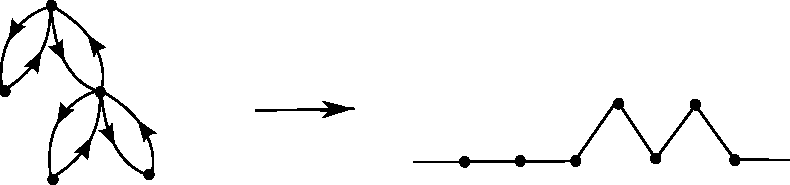
\includegraphics{Catalan-Pfad}
Lässt man die Wurzel außen vor, liegen \(r\ k\)-Knoten in den ungeraden Ebenen und \(l-r\ j\)-Knoten in den geraden Ebenen. Damit ergibt sich aus dieser Konstruktion, dass \(l-r\) die Anzahl der Aufstiege (und Abstiege) und \(2r\) die Anzahl der Flachstücke im Catalan-Pfad sind.  Denn: zu jedem \(j\)-Knoten führt genau eine Kante aus einer unteren Ebene hin und es führt genau eine Kante in eine untere Ebene zurück (Doppelbaum!). \\
\\ Die Abbildung von den Doppelbäumen auf die Catalanpfade ist eine Bijektion, da:
\begin{itemize}
 \item[•]Da der Graph eulersch ist, ist $ \sum_{i=1}^{2l} $ =0; Der Graph ist immer über 0, ansonsten würde es ein m geben, sodass $ \sum_{i=1}^{2m-1}s^{i}=-1, ~\sum_{i=1}^{2m}s^{i}=0, ~ s_{2m-1}=-1  $. Also könnten wir einen Doppelbaum mit Knoten {1,2,...2m} konstruieren, und da $ s_{2m-1}=-1  $ ist, würde eine Kante von diesem Knoten zurück zu einem der ersten 2m Knoten gehen, was dem Aufbau eines Doppelbaums widersprechen würde. Insgesamt haben wir also einen Catalanpfad konstruiert. 
 \item[•] Surjektivität:  für jeden Catalanpfad der Länge l der Form $\lbrace s_{i} \rbrace$, $ i \leq 2l, i \in \NN $ kann ein Doppelbaum als Urbild wie folgt konstruiert werden: für i gerade: $s_{i}=-1 \rightarrow $ gehe von $j_{i/2}$abwärts, bei $s_{i}=0  $ aufwärts; für i ungerade bei $s_{i}=1 $ aufwärts, bei $s_{i}=0 $ abwärts. 
\item[•] Injektivität analog zur Übung (bzw muss man das unbedingt nochmal zeigen?)\\
\end{itemize}
Die betrachteten Doppelbäume haben s.o. ein kombinatorisches Gewicht von 
	\[ \begin{pmatrix} N\\ l+1-r\end{pmatrix} (l+1-r)! \begin{pmatrix} M(N)\\r\end{pmatrix} r! \]
Für N hinreichend groß ist dies genähert \(N^{l+1-r}M(N)^r\). Damit folgt:
	\[\frac {1}{N^{l+1}} N^{l+1-r}M(N)^r =~ \left( \dfrac{M(N)}{N}\right)^{r}\to \alpha^r\]
und damit:
	\begin{align*}
		\beta_l &= \lim_{N \to \infty} \sum_{J,K: v(J)+v(K) = l+1} \dfrac{1}{N^{l+1}}\EE[Y_N(J,K)] = \sum_{r=1}^{l} \alpha^r\ \begin{pmatrix} 2l-2\\2r-2\end{pmatrix} C_{l-r} \\
		&= \sum_{r=1}^{l} \sum_{p_{r} \in C_{l}} \alpha^{r} = \sum_{p\in C_l} \alpha^r
	\end{align*}

wobei \(r = \frac 1 2 \#\{\text{Flachstücke in }C_l\} = l  - \#\{\text{Anstiege in }  C_l\}\), und $ p_{r} $ Catalanpfad mit r Flächenstücken.\\
$ l-r $ im Exponenten von $ \gamma_{l} $ sind die Aufstiege/Abstiege im Doppelbaum.\\


An Manu: kannst du diese Formel für \(\beta_l\) genauer erklären? Ich verstehe nicht wirklich, was du da machst...\\


Mach ich. Also ich hab lang nicht verstanden, was das Kombinatorik-zeug vorne dran mit den Catalanpfaden zu tun hat. Du hattest glaub ich $C_l$ als Anzahl der Catalanpfade. Beim Überlegen für (10) dem nächsten Punkt hab ich mir dann die Formel für die Pfade gebaut, die im Grunde nur auf deiner Konstruktion basiert (und von der bist du ja hoffentlich überzeugt:) )\\
$ \longrightarrow $Also wir brauchen die Anzahl der Catalanpfade, durch die wir unsere Doppelbäume beschreiben, weil's eine Bijektion ist. Nur haben wir andere Catalanpfade als die normalen:)\\
Die Catalanpfade, die wir in der Vorlesung gebaut haben, mit der Anzahl $C_l$ (Catalanzahlen), sind dadurch definiert, dass du bei jedem Schritt + oder - 1 gehst, und das nichtüberkreuzend. \\ Bei unseren Catalanpfaden hast du aber noch deine "Flachstücke" mit 0 eingebaut! Und zwar r von denen. Also wie viele gibts von denen für ein bestimmtes r? Nach Konstruktion mit einem Knoten, sagen wir mal den j1, als Wurzel, sind der erste und letzte Schritt in dem Pfad auf jeden Fall flach, also 0. Da gibt's keine andere Möglichkeit. Von den restlichen 2l-2 Schritten im Pfad sind noch r-2 flach, die suchen wir als erstes raus. Das macht dann die $\begin{pmatrix} 2l-2\\2r-2\end{pmatrix} $.\\ 
Bleiben uns noch l-2-(r-2) Schritte übrig, die mit +/-1 zu belegen sind. Und zwar nichtüberkreuzend. Was das gleiche ist wie wenn du einen l-r-langen Catalanpfad bauen willst, weil du die r Flachstücke einfach mal ignorierst, die ändern ja nichts. Daher kommt das $ C_{l-r} $. Und wir haben die Anzahl!\\ Über r aufsummieren, damit wir alle Fälle mit r Knoten aus M(N), Rest aus N, haben. Das übrige Kombinatorik-zeug ist ja $\alpha^r  $, und schon steht die Formel da\\
Die Formel für die Anzahl der Catlanpfade ist ganz praktisch für (10), für $ \beta$ selber brauchen wir sie ja erst mal nicht, deshalb wieder umcshreiben in $ \sum_{r} \alpha^{r} \#\{ \text{Catalanpfade mit r Flachstücke} \}$. Wenn du sie mal die Anzahl nimmst, kannst auch über alle r-Catalanpfade aufsummieren, das hoch r ändert sich ja nicht. Und dann $= \sum_{r=1}^{l} \sum_{p_{r} \in C_{l}} \alpha^{r} = \sum_{p\in C_l} \alpha^r $.\\ \\
Jetzt verständlicher? Oder stimmt was nicht? Aber zumindest der erste Teil von (10) funktioniert ja gut mit der Formel, das sollte also schon passen. Sorry dass ich erst jetzt dazu gekommen bin, das zu schreiben. kurze Erklärung der Schritte schreib ich auch noch irgendwann oben rein.\\




%Induktionsanfang: \(l=1\): 
	%\[\beta_1 = \alpha\gamma_1=\alpha\beta_0 \gamma_0=\alpha\]
	
%Induktionsschritt: Ich denke, dass aus der Rekursionsformel für Catalanzahlen \(C_{l+1} = \sum_{k=0}^l C_kC_{l-k}\) folgt, dass
	%\[\beta_{l+1} = \sum_{k=0}^l \beta_k\beta_{l-k} = \alpha \sum_{k=0}^l \beta_k\gamma_{l-k}\]
%aber das ist eher wage...

\textbf{Beweis von  $\beta_{l}= \alpha \gamma_{l}$:}
\begin{align*}
\alpha \gamma_{l} =& \sum_{p \in C_l} \alpha^{l+1-r},\\
\beta_l - \alpha \gamma_l =& \sum_{r=1}^{l} \alpha^r\ \begin{pmatrix} 2l-2\\2r-2\end{pmatrix} C_{l-r} - \sum_{r=1}^{l} \alpha^{l+1-r}\ \begin{pmatrix} 2l-2\\2l-2r\end{pmatrix} C_{r-1}   \\ 
\underset{\text{Symmetrie Binom.}}{=}& \sum_{r=1}^{l} \begin{pmatrix} 2l-2\\2l-2r\end{pmatrix} \left( C_{l-r} \alpha^r - C_{r-1}\alpha^{l+1-r} \right) \\
\overset{!}{=}& 0 \\
\end{align*}
Für die einzelnen Summenglieder folgt:
\begin{align*}
\text{i-tes Summenglied:} &\begin{pmatrix} 2l-2\\2l-2i\end{pmatrix} \left( C_{l-i} \alpha^i - C_{i-1}\alpha^{l+1-i} \right) \\
\text{(l+1-i)-tes Summenglied:}& \begin{pmatrix} 2l-2\\2l-2-2l+2i\end{pmatrix} \left( C_{l-1-l+i} \alpha^{l+1-i} - C_{1+l-i-1}\alpha^{l+1-1-l+i} \right)\\
 &= - \text{i-tes Summenglied}  
\end{align*}
Ist l gerade, dann heben sich folglich alle Summenglieder weg und die Summe ist 0, ist l ungerade, bleibt nur das (l+1)/2-te Summenglied übrig:
\begin{align*}
 &\begin{pmatrix} 2l-2\\l+1-2\end{pmatrix} \left( C_{l-\frac{l+1}{2}} \alpha^{\frac{l+1}{2}} - C_{\frac{l+1}{2} -1}\alpha^{l+1-\frac{l+1}{2}} \right)\\
&=\begin{pmatrix} 2l-2\\l-1\end{pmatrix} \left( C_{\frac{l-1}{2}} \alpha^{\frac{l+1}{2}} - C_{\frac{l-1}{2}}\alpha^{\frac{l+1}{2}} \right)=0
\end{align*}

Fehlt noch Beweis der zweiten Hälfte von (10), da komm ich nicht weiter.\\
Danke für die Formatierung :) aber Latex soll sich nicht so anstellen nur weil die Formeln ein bisschen lang sind..\\



\textbf{Beweis Formel (12)}\\
\begin{align*}
	Q_n =& \alpha^{-1-n/2}\int_{\RR} f_{\alpha}(x)x(x-\alpha -1)^n\,\mathrm{d}x \\
	 =& \frac{1}{2\pi}\alpha^{-1-n/2} \int_{(1-\sqrt{\alpha})^2}^{(1+\sqrt{\alpha})^2} \sqrt{(x-(1-\sqrt{\alpha})^2)((1+\sqrt{\alpha})^2-x)} (x-\alpha -1)^n \,\mathrm{d}x\\
	=& \frac{1}{2\pi}\alpha^{-1-n/2} \int_{(1-\sqrt{\alpha})^2}^{(1+\sqrt{\alpha})^2} \sqrt{-\alpha^2+2\alpha x+2\alpha -x^2+2x-1}(x-\alpha-1)^n \,\mathrm{d}x\\
	\overset{x=y+\alpha+1}{=}& \frac{1}{2\pi}\alpha^{-1-n/2} \int_{-2\sqrt{\alpha}}^{2\sqrt{\alpha}} \sqrt{4\alpha -y^2} y^n \,\mathrm{d}y\\
	\overset{y=2\sqrt{\alpha}z}{=}& \frac{1}{2\pi}\alpha^{-1-n/2} \cdot 2^n \alpha^{n/2}\cdot4\sqrt{\alpha}\int_{-1}^{1} \sqrt{1-z^2}z^n \,\mathrm{d}z = \frac{2}{\pi} \cdot 2^n\int_{-1}^{1} \sqrt{1-z^2}z^n\,\mathrm{d}z \\
	\overset{\text{Übung 1}}{=}& \sigma(z^n) = \begin{cases} 0, &n\text{ ungerade}\\
	C_{\frac l 2}, &n\text{gerade} \end{cases}
\end{align*}
(Falls wir noch Platz füllen müssen, können wir hier die Rechnung aus der Übung auch wiederholen ;) )
Bei den "`Verständnis-Fragen"' habe ich jedoch etwas Probleme: \(f_{\alpha}\) ist für x=0 gar nicht definiert? Durch die Rechnung ergibt sich aber der Bezug zu \(\sigma(x)\), wo man dann doch beim Halbkreisgesetz wäre.\\
Zur Eindeutigkeit von \(f_{\alpha}\) sind diese "`verallgemeinerten Momente"' ein Problem. Habt ihr in der großen W-Theorie Vorlesung dazu was gemacht?



\end{beweis}


\end{document}
